\section{Introduction}
\label{sec:introduction}
\begin{figure}[t]
  \centering
  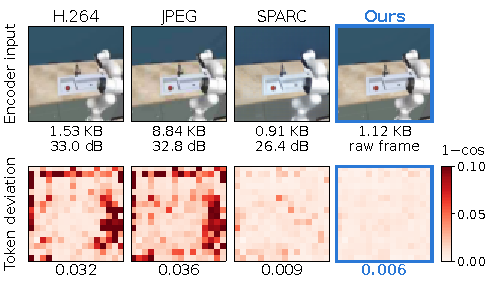
\includegraphics[width=\columnwidth]{images/pixel-vs-control.pdf}
  \caption{Pixel fidelity is not control fidelity. On RoboCasa, H.264
  frames at 3.0\,KB per upload look close to the originals, yet
  $\pi_{0.5}$ succeeds in 0 of 480 episodes; the policy tokens computed
  from them deviate most around the robot arm. Our frontend sends
  1.14\,KB per upload, recovers tokens close to the clean ones, and
  succeeds in 295 of 480 episodes (uncompressed: 291). Deviation is
  $1-\cos$ between each post-projection policy token and its clean
  counterpart, overlaid on a lightened copy of the original frame. The
  upload shown has the median H.264 deviation in its episode; across all
  24 uploads and three cameras of that episode, H.264 deviation averages
  $4.0\times$ ours.}
  \Description{Four square panels of a simulated kitchen with a robot arm.
  The original frame and the H.264 frame look almost identical. A heatmap
  of token deviation for H.264 is bright around the robot arm and at some
  image borders, with mean 0.032. The same heatmap for our frontend is
  almost dark, with mean 0.006.}
  \label{fig:pixel-vs-control}
\end{figure}
% TODO(author): replace the single-episode ratio (4.0x) with the held-out
% 8-episode average once computed.

A robot using a remotely hosted vision--language--action (VLA) policy must
repeatedly send visual observations and receive actions while its physical
state continues to change. Models such as $\pi_{0.5}$ and OpenVLA use
visual observations and language to support manipulation
tasks~\cite{pi05,openvla}. OpenVLA-OFT studies how adaptation and action
decoding affect both speed and success~\cite{openvlaoft}. In an edge--cloud
deployment, these capabilities depend on more than policy inference
alone. The robot must prepare its observations, transfer them, and wait
for the cloud to process them. Our SO-101 deployment makes this division
concrete: an Orin device processes camera inputs while an A40 server
hosts the policy. Work added to either side recurs with each new visual
request.

Image offloading and model partitioning address different parts of this
cost. Progressive image transmission, exemplified by LimitNet, targets
vision offloading under constrained device and network
resources~\cite{limitnet}. SPARC goes further for VLA policies by using
action-aware image compression and temporal masking~\cite{sparc}.
These approaches still recover images before the policy's visual
processing. Image fidelity, however, is a poor proxy for what the policy needs:
H.264 frames that look nearly unchanged can make the policy fail in every
episode (Figure~\ref{fig:pixel-vs-control}). Collaborative inference systems instead choose where model
computation runs~\cite{neurosurgeon,roboecc,rapid}, while feature
communication methods such as BottleNet++ compress intermediate
representations~\cite{bottlenetpp}. For a robot, moving a full visual
encoder to the edge can trade network traffic for local computation.
Consequently, a smaller payload alone does not establish a faster
deployment, and the best division of work depends on the representation
that crosses the network.

We study a visual communication interface that recovers the tokens
consumed by a frozen VLA policy. A lightweight encoder on the robot
produces a discrete feature stream, and a cloud decoder supplies the
policy's visual inputs without reconstructing an intermediate image.
For our primary $\pi_{0.5}$ configuration, the receiver replaces the
original visual tower and projection. This choice changes both the
communication payload and the computation required to consume it. Our
goal is to make this interface useful on a constrained edge device while
limiting its effect on control quality. We evaluate it against the
original policy under the same task conditions rather than treating
differences between policy backbones as compression gains.

Three obstacles shape the design. First, feature similarity is an
incomplete proxy for action quality: a compact representation must retain
information needed by the downstream controller. Second, the edge encoder
must be cheap enough that its work does not erase savings in communication
or cloud processing. Third, temporal coding must keep the sender and
receiver consistent without requiring a neural reconstruction decoder on
the robot. These obstacles concern the representation, the local
computation, and the state carried across uploads. Measuring their
combined effect also requires distinguishing visual-path microbenchmarks,
complete request latency, and physical task outcomes.

Our design combines policy supervision, a distilled visual tower, and
temporal coding over quantized features. Clean-input tokens and actions
from the original policy supervise the trainable student and codec while
the policy weights stay frozen. A compact student reduces visual
encoding work relative to running the original tower on the robot,
following the use of teacher supervision
for model compression~\cite{distillation}. Quantized code references
support temporal prediction, and integer rANS turns the resulting symbols
into a deployable bitstream~\cite{ans}. The cloud reconstructs policy
tokens directly. We implement the main path for $\pi_{0.5}$ and adapt
the student and decoder interface to OpenVLA-OFT. Each policy requires
its own training; the design does not assume that a single codec can
serve arbitrary VLA backbones.

This paper contributes a policy-aligned feature interface and its
training design (\S\ref{sec:overview}--\S\ref{sec:design-objective}), a
temporal bitstream implementation that avoids neural decoding at the
edge (\S\ref{sec:design-temporal}--\S\ref{sec:implementation}), and an
empirical characterization of the quality--cost tradeoff
(\S\ref{sec:evaluation}). The current evidence includes paired simulation
results and recorded-observation replay through a real edge--cloud stack.
It also identifies limits: the confidence intervals do not establish
lossless control, SPARC can use fewer bytes, stronger cloud hardware can
reduce the latency advantage, and shifted visual conditions can lower
success. These boundaries motivate evaluating a communication interface
as part of a control system rather than ranking codecs by payload alone.
